\section{Risultati}


% PEAK SWE
\begin{frame}{Peak SWE trend}

  \begin{columns}[c, onlytextwidth]

    \begin{column}{0.52\textwidth}
      \centering
      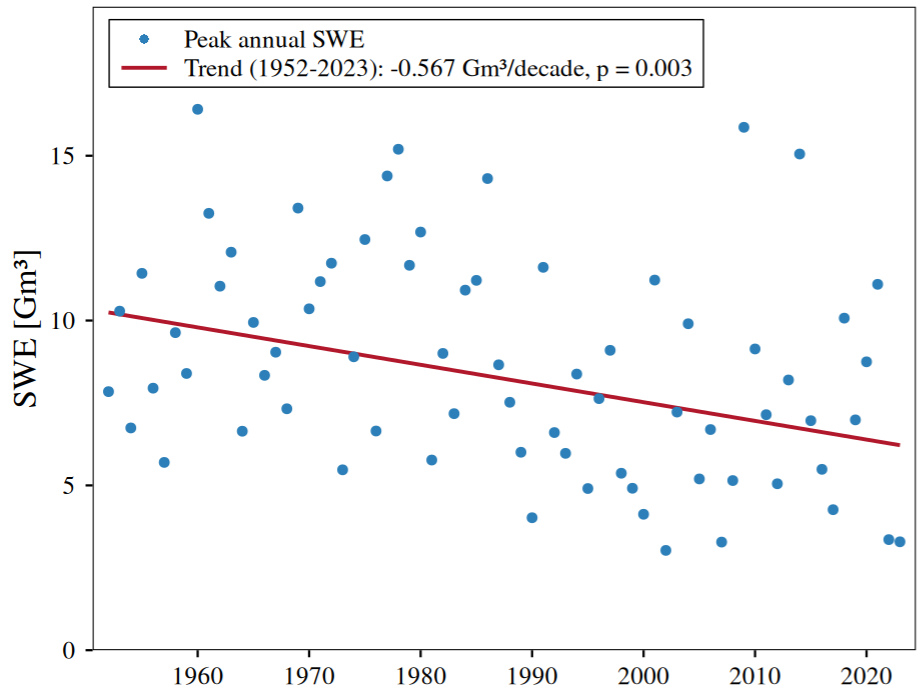
\includegraphics[width=\linewidth, height=0.8\textheight, keepaspectratio]{images/results/trend_peak_SWE.png}\\[2pt]
    \end{column}

    \begin{column}{0.45\textwidth}
      \centering
      {\usebeamercolor[fg]{structure}\small\bfseries Elevation-wise peak SWE trend\par}
      \smallskip
      \footnotesize
      \renewcommand{\arraystretch}{1.2}
      \setlength{\tabcolsep}{5pt}   % spazio tra le colonne: riducilo se la tabella è troppo larga
      \begin{tabular}{@{}cc@{}}
        \toprule
        Quota [m]   & Trend [\%/decade] \\
        \midrule
        0--500      & $-8.6$ \\
        500--1000   & $-8.7$ \\
        1000--1500  & $-6.3$ \\
        1500--2000  & $-5.7$ \\
        2000--2500  & $-5.2$ \\
        $>$2500     & $-3.6$ \\
        \bottomrule
      \end{tabular}\\[6pt]
    \end{column}

  \end{columns}

  \vspace{0.75cm} 
  \begin{columns}[T, onlytextwidth]
    \begin{column}{0.31\textwidth}
      \centering
      {\usebeamercolor[fg]{structure}\large\bfseries\boldmath $-$35/40\%\par}
      {\footnotesize peak SWE in 72 anni\par}
    \end{column}
    \begin{column}{0.31\textwidth}
      \centering
      {\usebeamercolor[fg]{structure}\large\bfseries\boldmath 7.4 $\text{Gm}^3$\par}
      {\footnotesize picco medio 1991--2020\\2 Marzo\par}
    \end{column}
    \begin{column}{0.31\textwidth}
      \centering
      {\usebeamercolor[fg]{structure}\large\bfseries \smallleq{} 1000\,m\par}
      {\footnotesize fascia di quota più colpita\par}
    \end{column}
  \end{columns}
\end{frame}


% VARIAZIONI STAGIONALI
\begin{frame}{Variazioni stagionali}

  \begin{columns}[c, onlytextwidth]

    \begin{column}{0.7\textwidth}
      \centering
      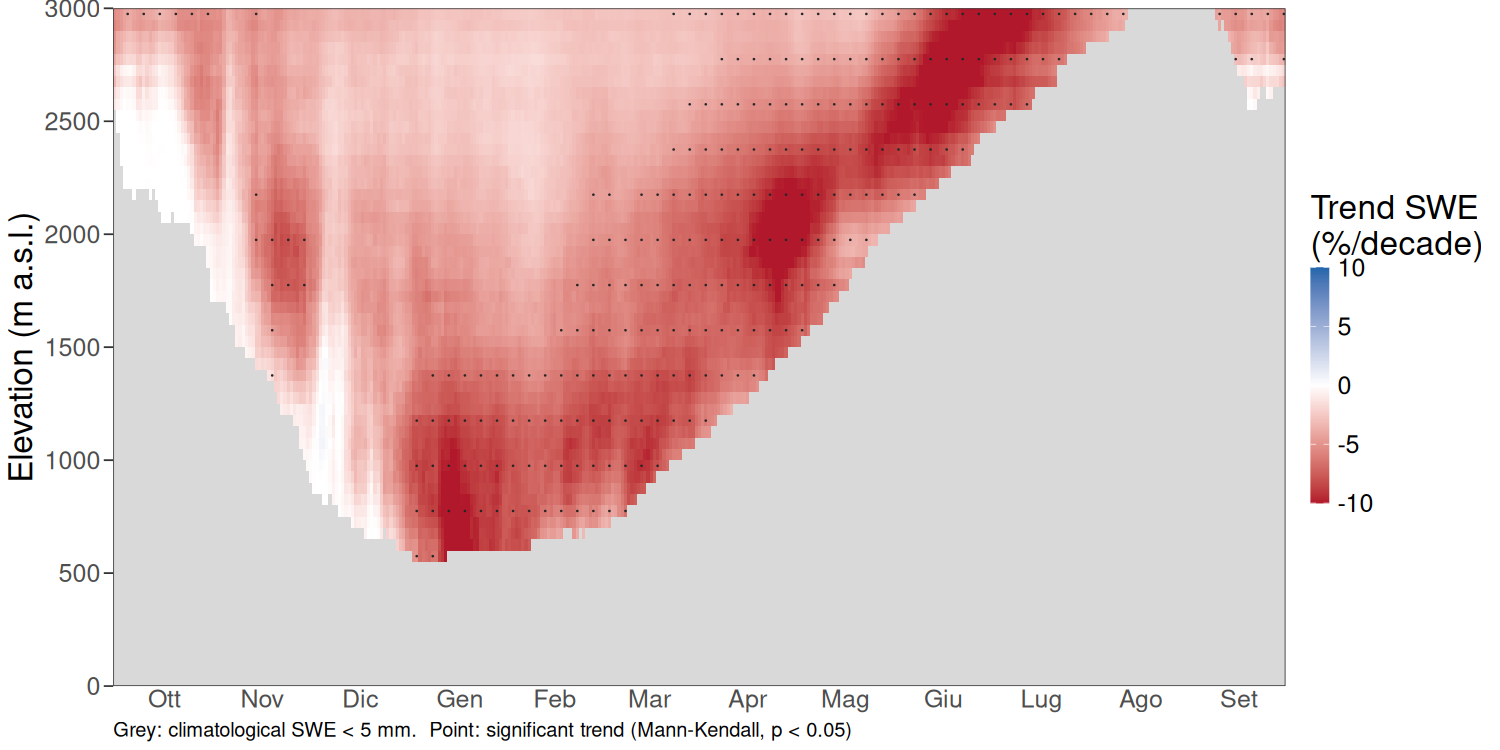
\includegraphics[width=\linewidth, height=\textheight, keepaspectratio]{images/results/trend_by_ele_by_date.png}\\
    \end{column}

    \begin{column}{0.3\textwidth}
      \centering
      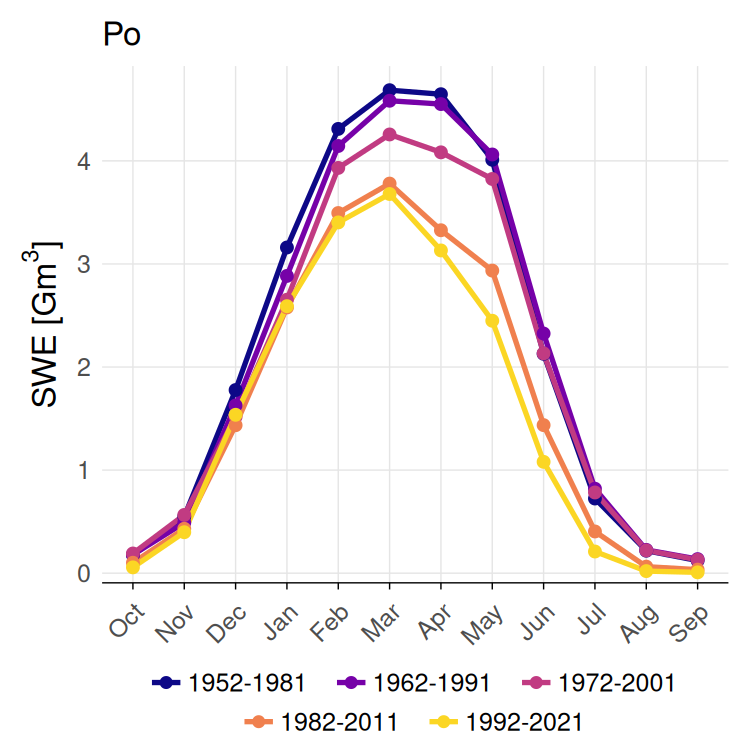
\includegraphics[width=\linewidth, height=\textheight, keepaspectratio]{images/results/swe_clima_po.png}\\
    \end{column}

  \end{columns}

  \vspace{0.75cm} 
  \begin{columns}[T, onlytextwidth]
    \begin{column}{0.31\textwidth}
      \centering
      {\usebeamercolor[fg]{structure}\large\bfseries\boldmath $<$1500 m\par}
      {\footnotesize perdite notevoli e sempre significative\par}
    \end{column}
    \begin{column}{0.31\textwidth}
      \centering
      {\usebeamercolor[fg]{structure}\large\bfseries\boldmath $>$ 1500 m\par}
      {\footnotesize perdite maggiori nei mesi primaverili\par}
    \end{column}
    \begin{column}{0.31\textwidth}
      \centering
      {\usebeamercolor[fg]{structure}\large\bfseries $\approx$ 1 mese\par}
      {\footnotesize anticipo fusione completa nei bacini idrici\par}
    \end{column}
  \end{columns}
\end{frame}


% SCD
\begin{frame}[t]{Snow cover duration}

  {\centering
  \begin{minipage}{0.45\textwidth}
    \begin{block}{SWE $\Rightarrow$ copertura nevosa}
      \centering
      \footnotesize
      Pixel innevato $\Leftrightarrow$ $\text{SWE} \geq 15$~mm w.e.
    \end{block}
  \end{minipage}
  \par}

  \vspace{2em}

  \begin{columns}[T, onlytextwidth]

    \begin{column}{0.48\textwidth}
      \centering
      {\usebeamercolor[fg]{structure}\bfseries Climatologia 1991--2020\par}
      \vspace{4pt}
      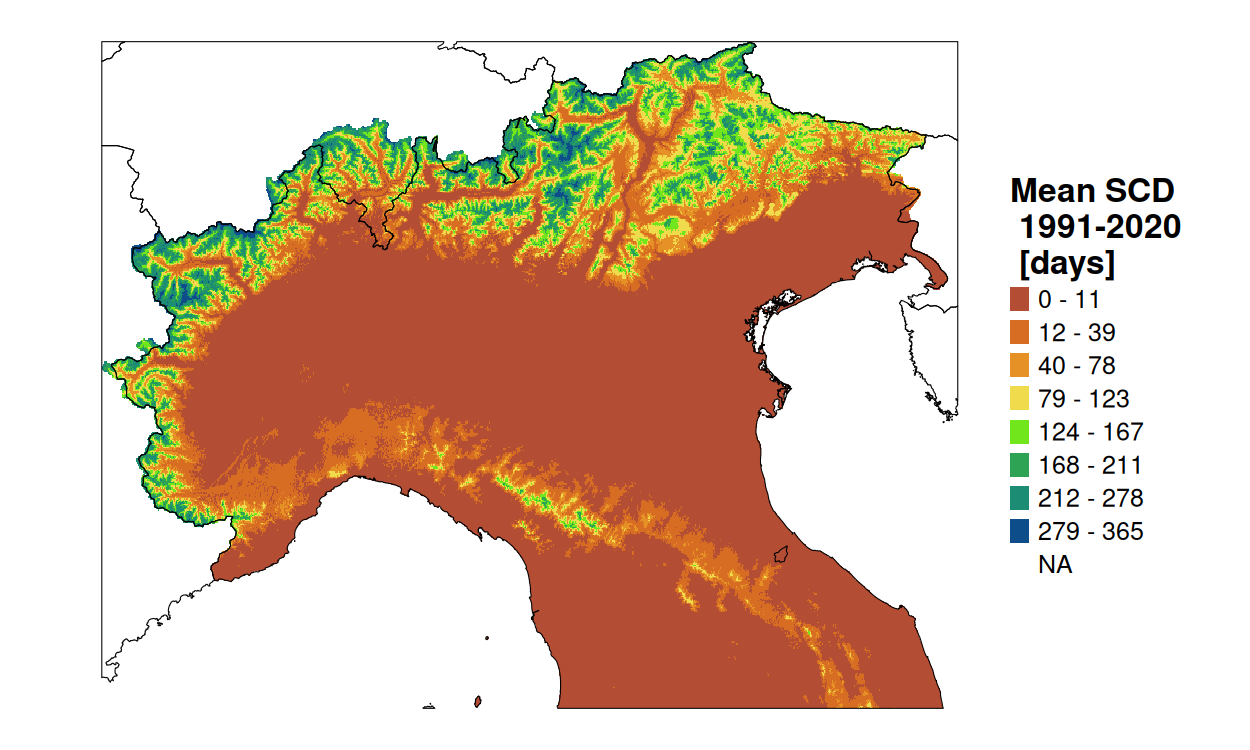
\includegraphics[width=\linewidth, height=0.48\textheight, keepaspectratio]{images/results/clima_scd_map_1991_2020.png}\par
      \vspace{4pt}
      {\scriptsize $\text{Quota} \nearrow \;\Rightarrow\; \text{SCD} \nearrow$\par}
    \end{column}

    \begin{column}{0.48\textwidth}
      \centering
      {\usebeamercolor[fg]{structure}\bfseries Trend 1952--2023\par}
      \vspace{4pt}
      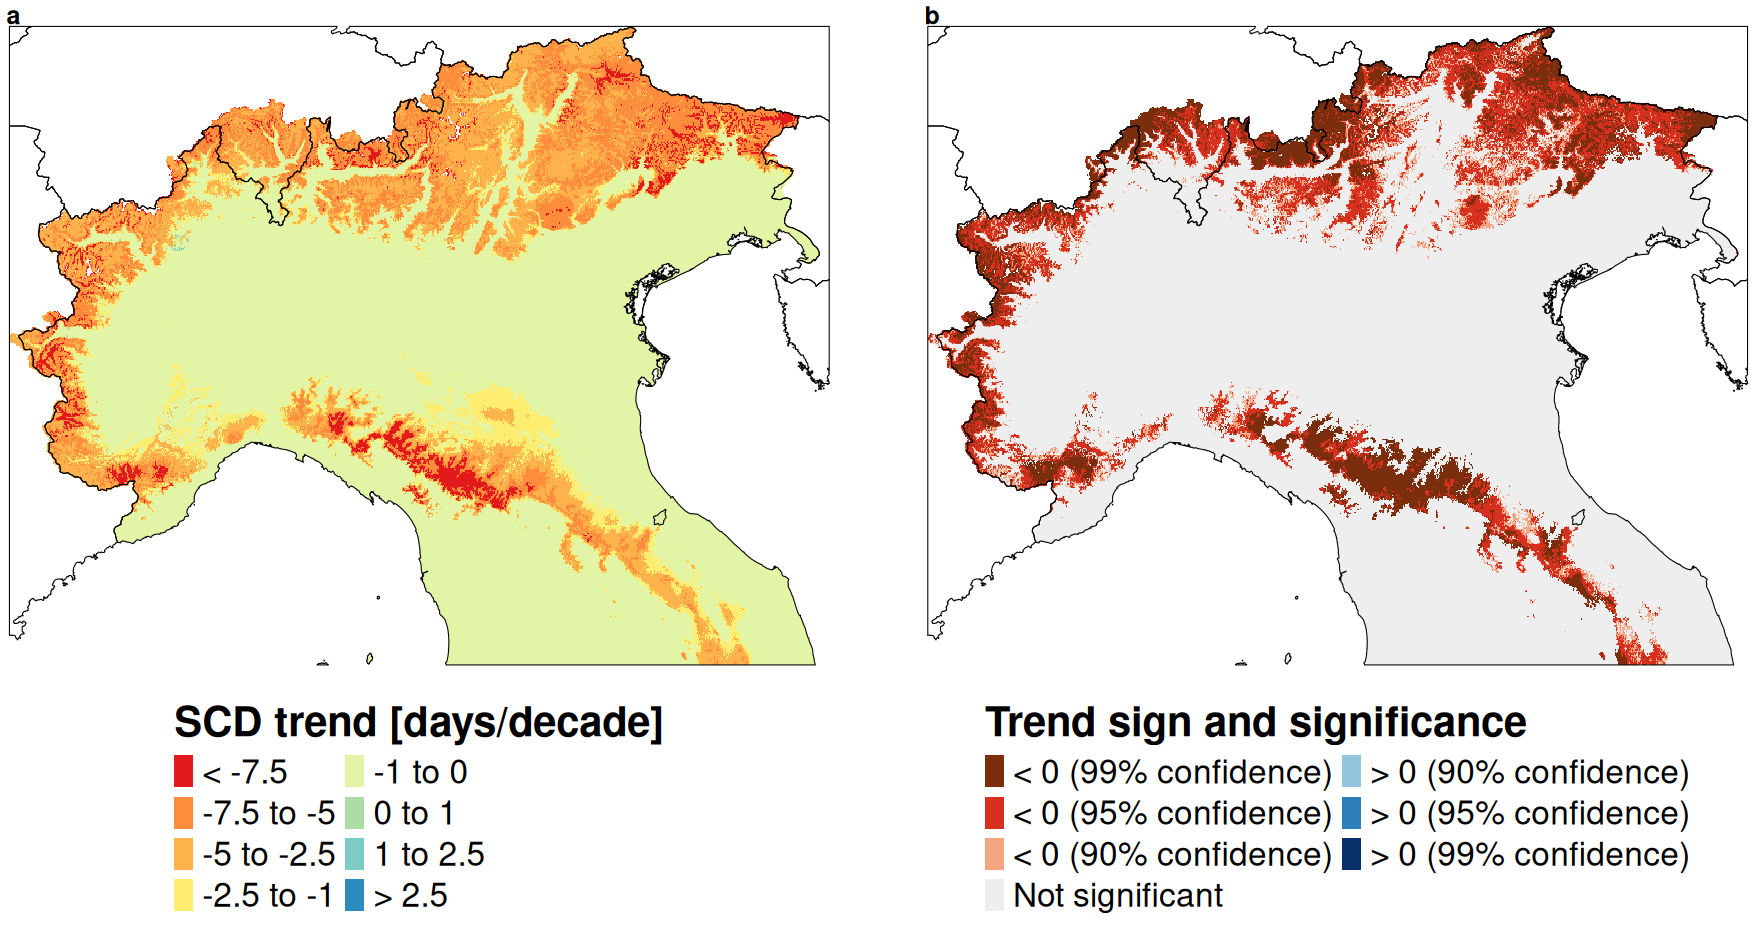
\includegraphics[width=\linewidth, height=0.48\textheight, keepaspectratio]{images/results/SCD_trends.png}\par
      \vspace{4pt}
      {\scriptsize Trend negativi significativi in ogni catena montuosa\par}
    \end{column}

  \end{columns}
\end{frame}


% CONFRONTO CON PRODOTTI SWE
\begin{frame}[t]{Confronto con prodotti SWE}

  \vspace{0.5em}

  \begin{columns}[T, onlytextwidth]

    \begin{column}{0.48\textwidth}
      \centering
      {\usebeamercolor[fg]{structure}\bfseries Po River District\par}
      {\footnotesize 1992--2021 \quad picco medio: 6.5 vs 4.5\,Gm$^3$}\par\smallskip
      
      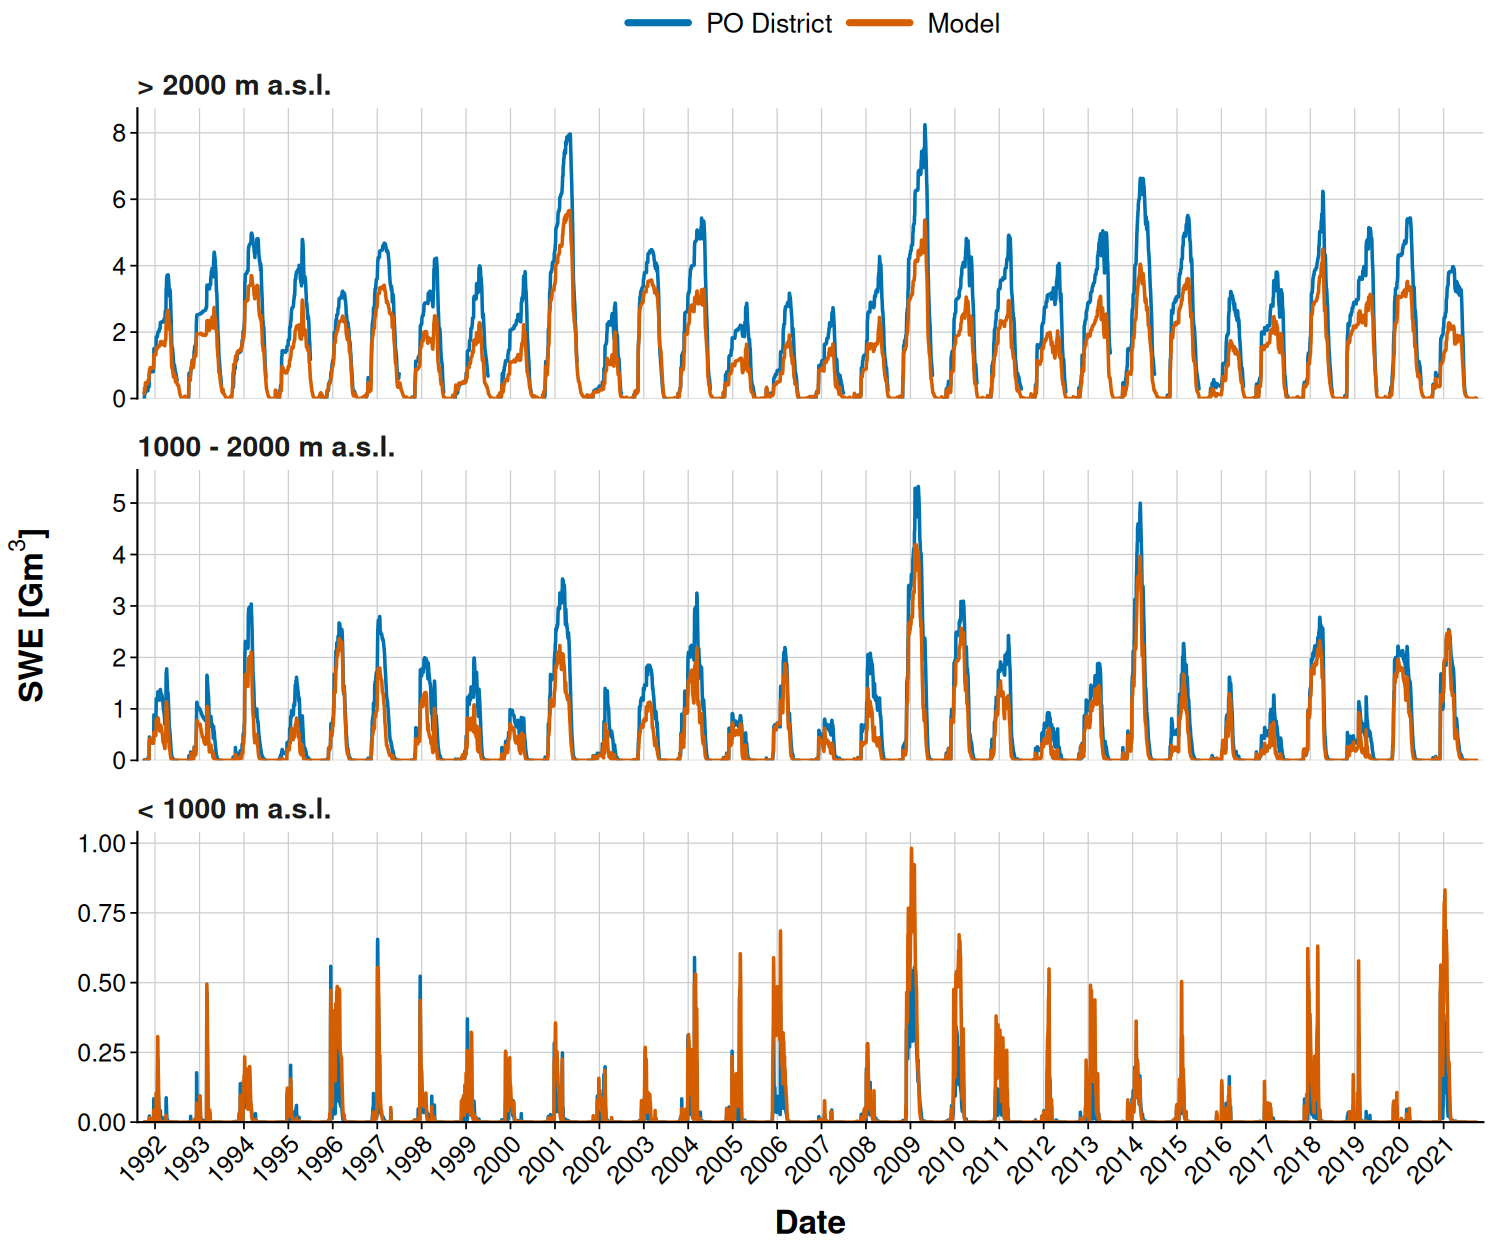
\includegraphics[width=\linewidth, height=0.7\textheight, keepaspectratio]{images/results/swe_evo_comparison_with_PO_basin.png}\par
    \end{column}

    \begin{column}{0.48\textwidth}
      \centering
      {\usebeamercolor[fg]{structure}\bfseries IT-SNOW\par}
      {\footnotesize 2011--2023 \quad picco medio: 10.7 vs 6.4\,Gm$^3$}\par\smallskip
      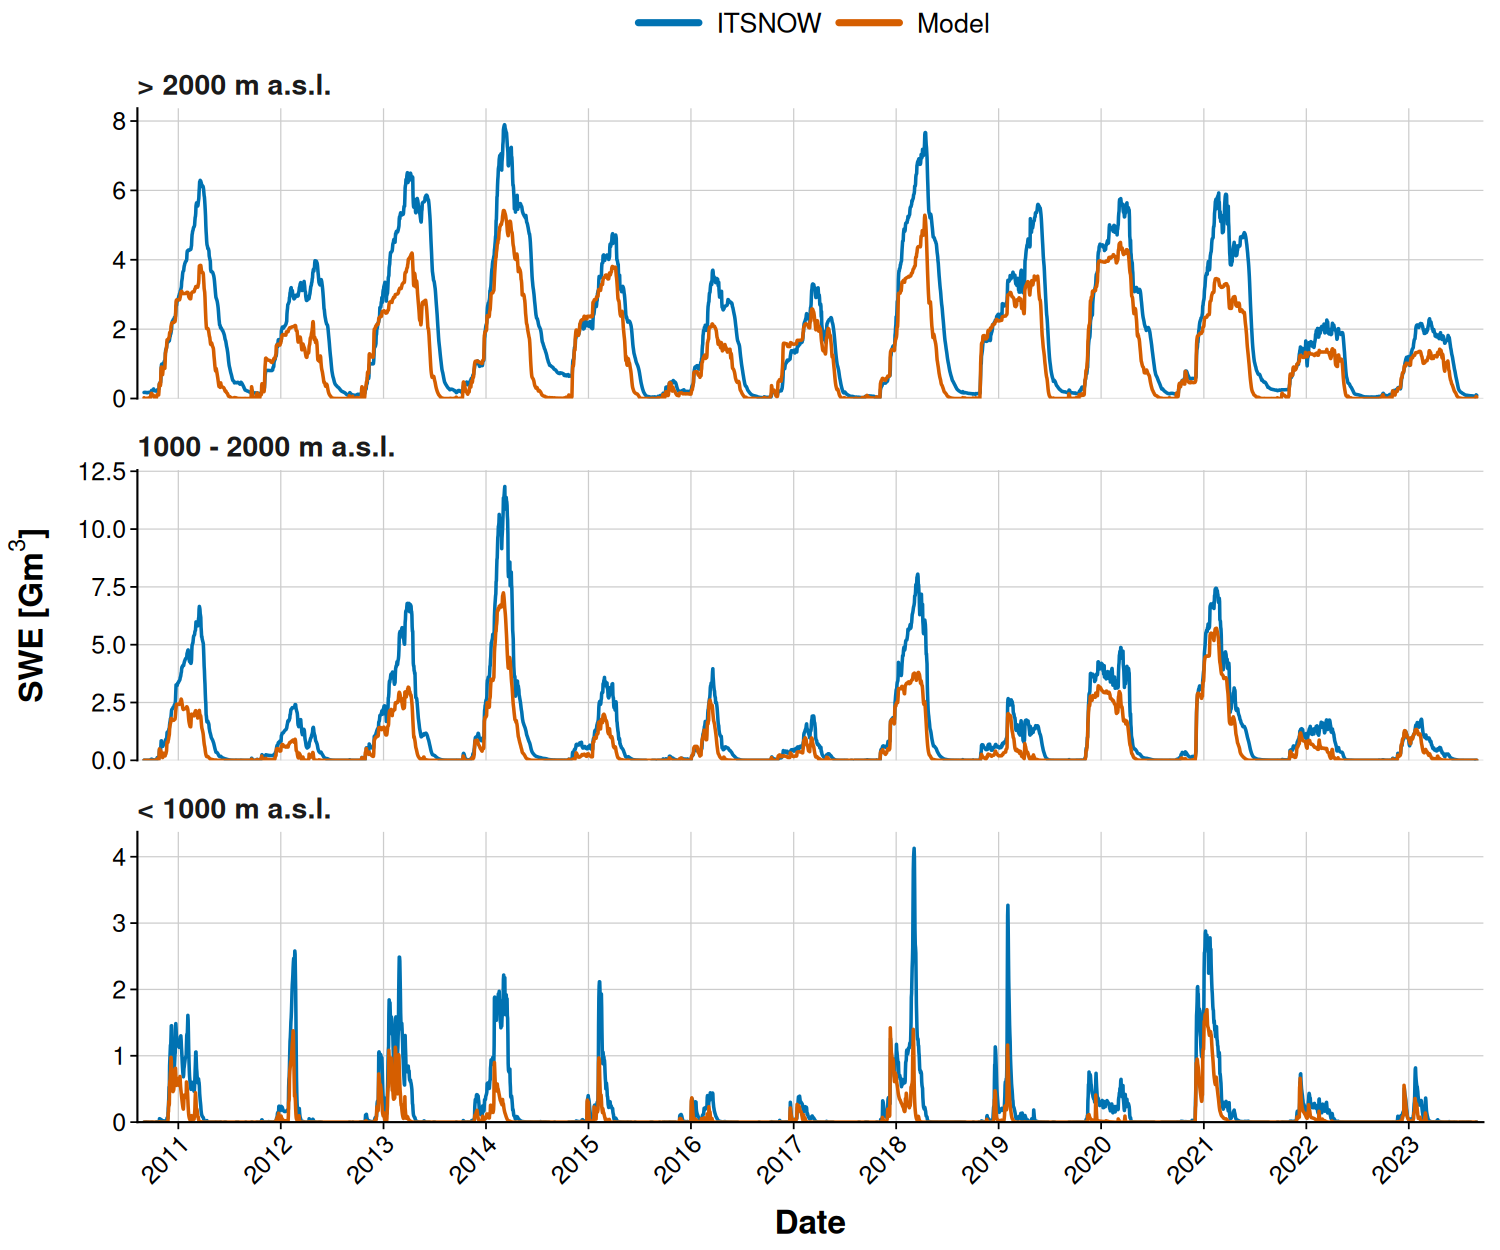
\includegraphics[width=\linewidth, height=0.7\textheight, keepaspectratio]{images/results/swe_evo_comparison_with_ITSNOW.png}\par
    \end{column}

  \end{columns}

  \vspace{8pt}
  \centering\small
  Variabilità interannuale ben riprodotta,
  ma SWE sottostimato in quota.\\
\end{frame}